\section{Overall Description}\label{sec:overall_desc}

\subsection{Product Perspective}

Customers Line-Up is developed for both shop managers and customers.
The intent is to provide functionalities adding value to the interactions between the two.
Managers have access to a website that will help them to avoid large crowds inside and outside their stores, providing them with useful analytics.
Customers may avoid queues by booking visits to stores via website or mobile application, and will be guided in selectiong the best place and time.
Customers must register an account in order to utilize the website or the mobile app.
Customers who do not possess an Internet-connected device may still utilize the service via physical totems outside the stores.

The system will be developed from scratch, giving great flexibility and scalability.
The privacy of the customers will be guaranteed according to the latest privacy related norms.

\subsubsection{Entities diagram}
\begin{figure}[H]
    \centering
    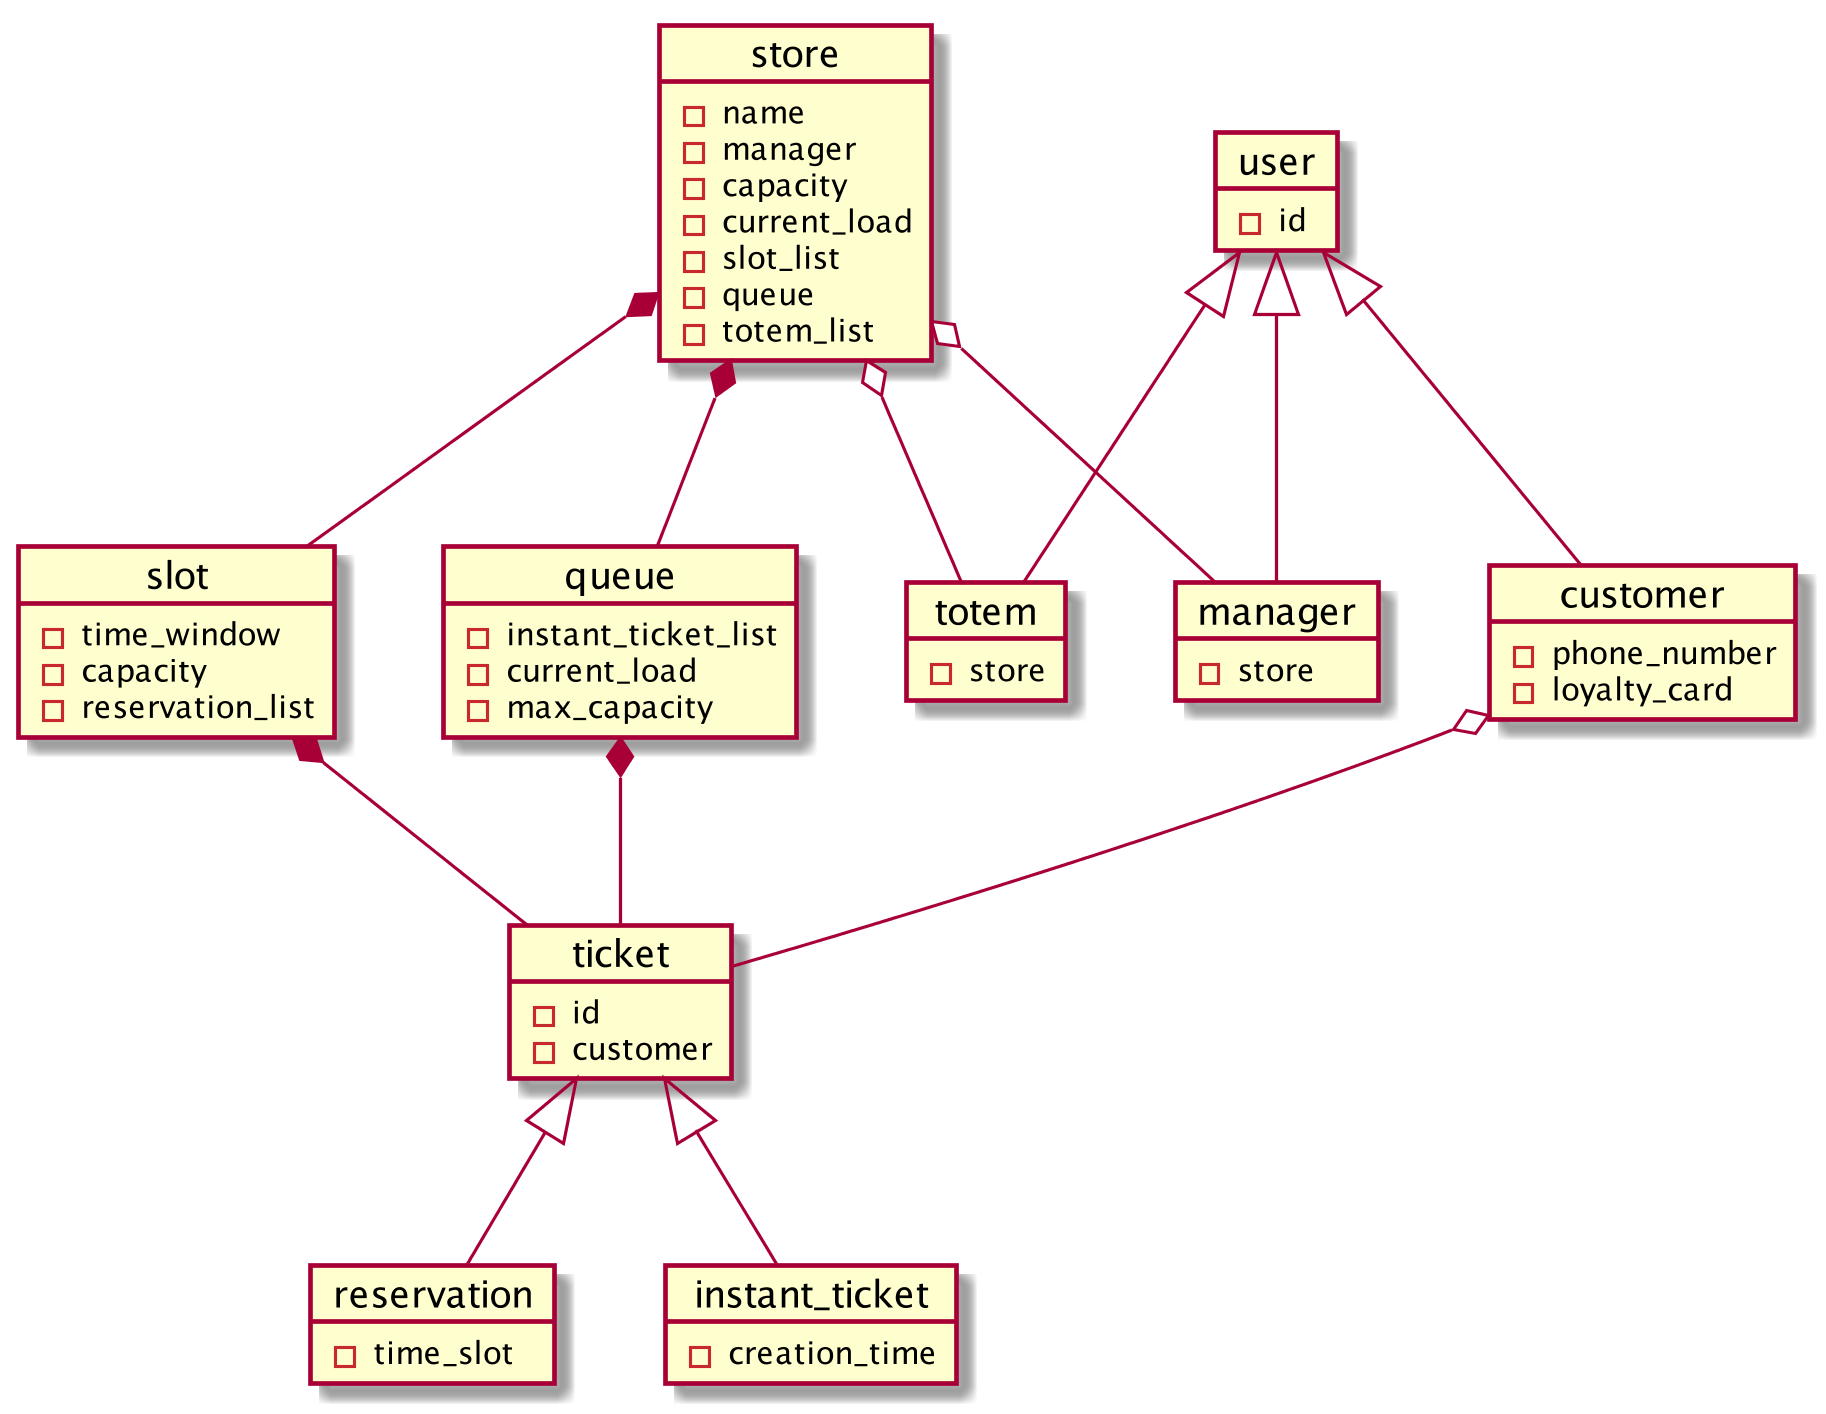
\includegraphics[width=1\textwidth]{uml/high_level_UML.png}
    \label{fig:high_UML}
    \caption{High level view of the main entities of the system}
\end{figure}


\subsubsection{State Diagrams}
\begin{figure}[H]
    \centering
    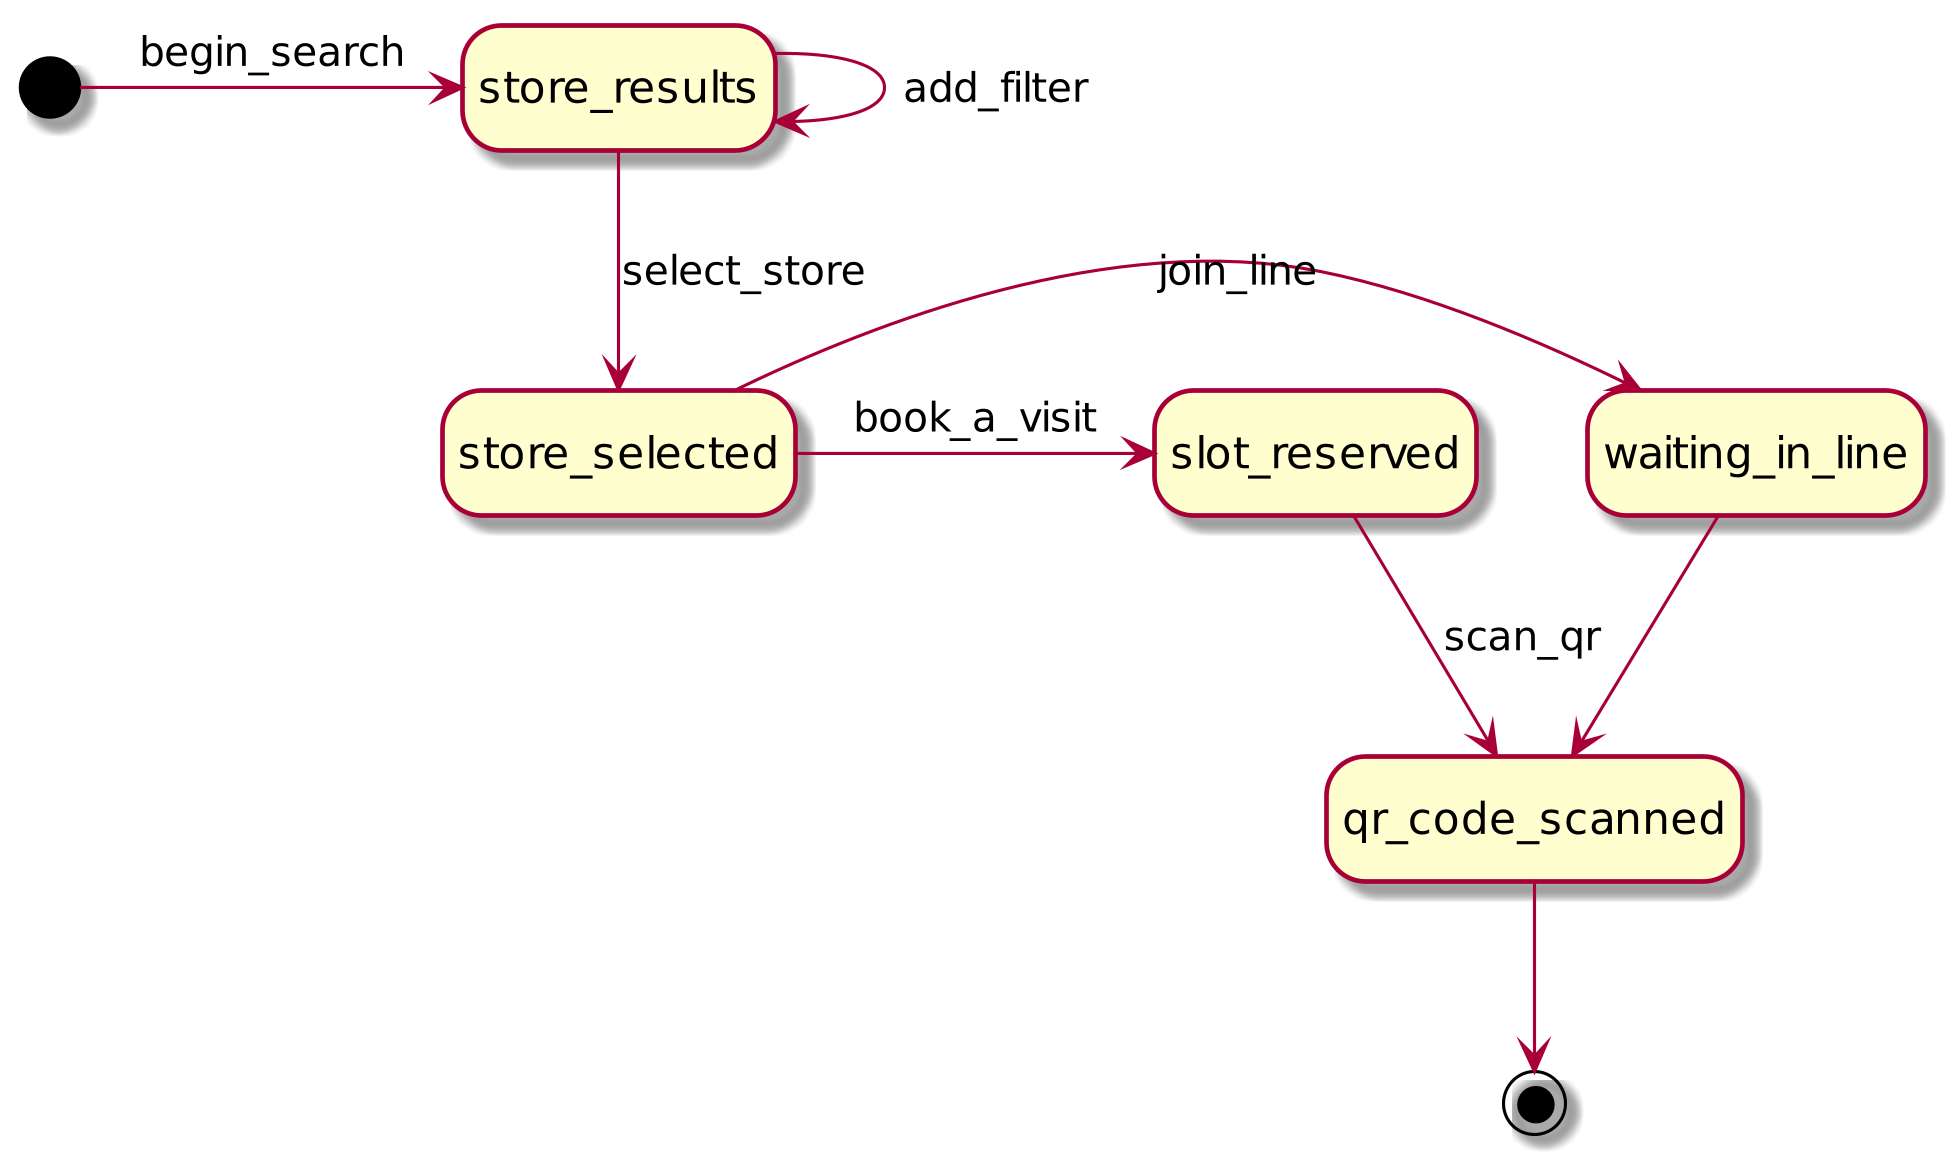
\includegraphics[width=1\textwidth]{uml/client_state_chart.png}
    \label{fig:client_state_diag}
    \caption{Client state diagram}
\end{figure}

\begin{figure}[H]
    \centering
    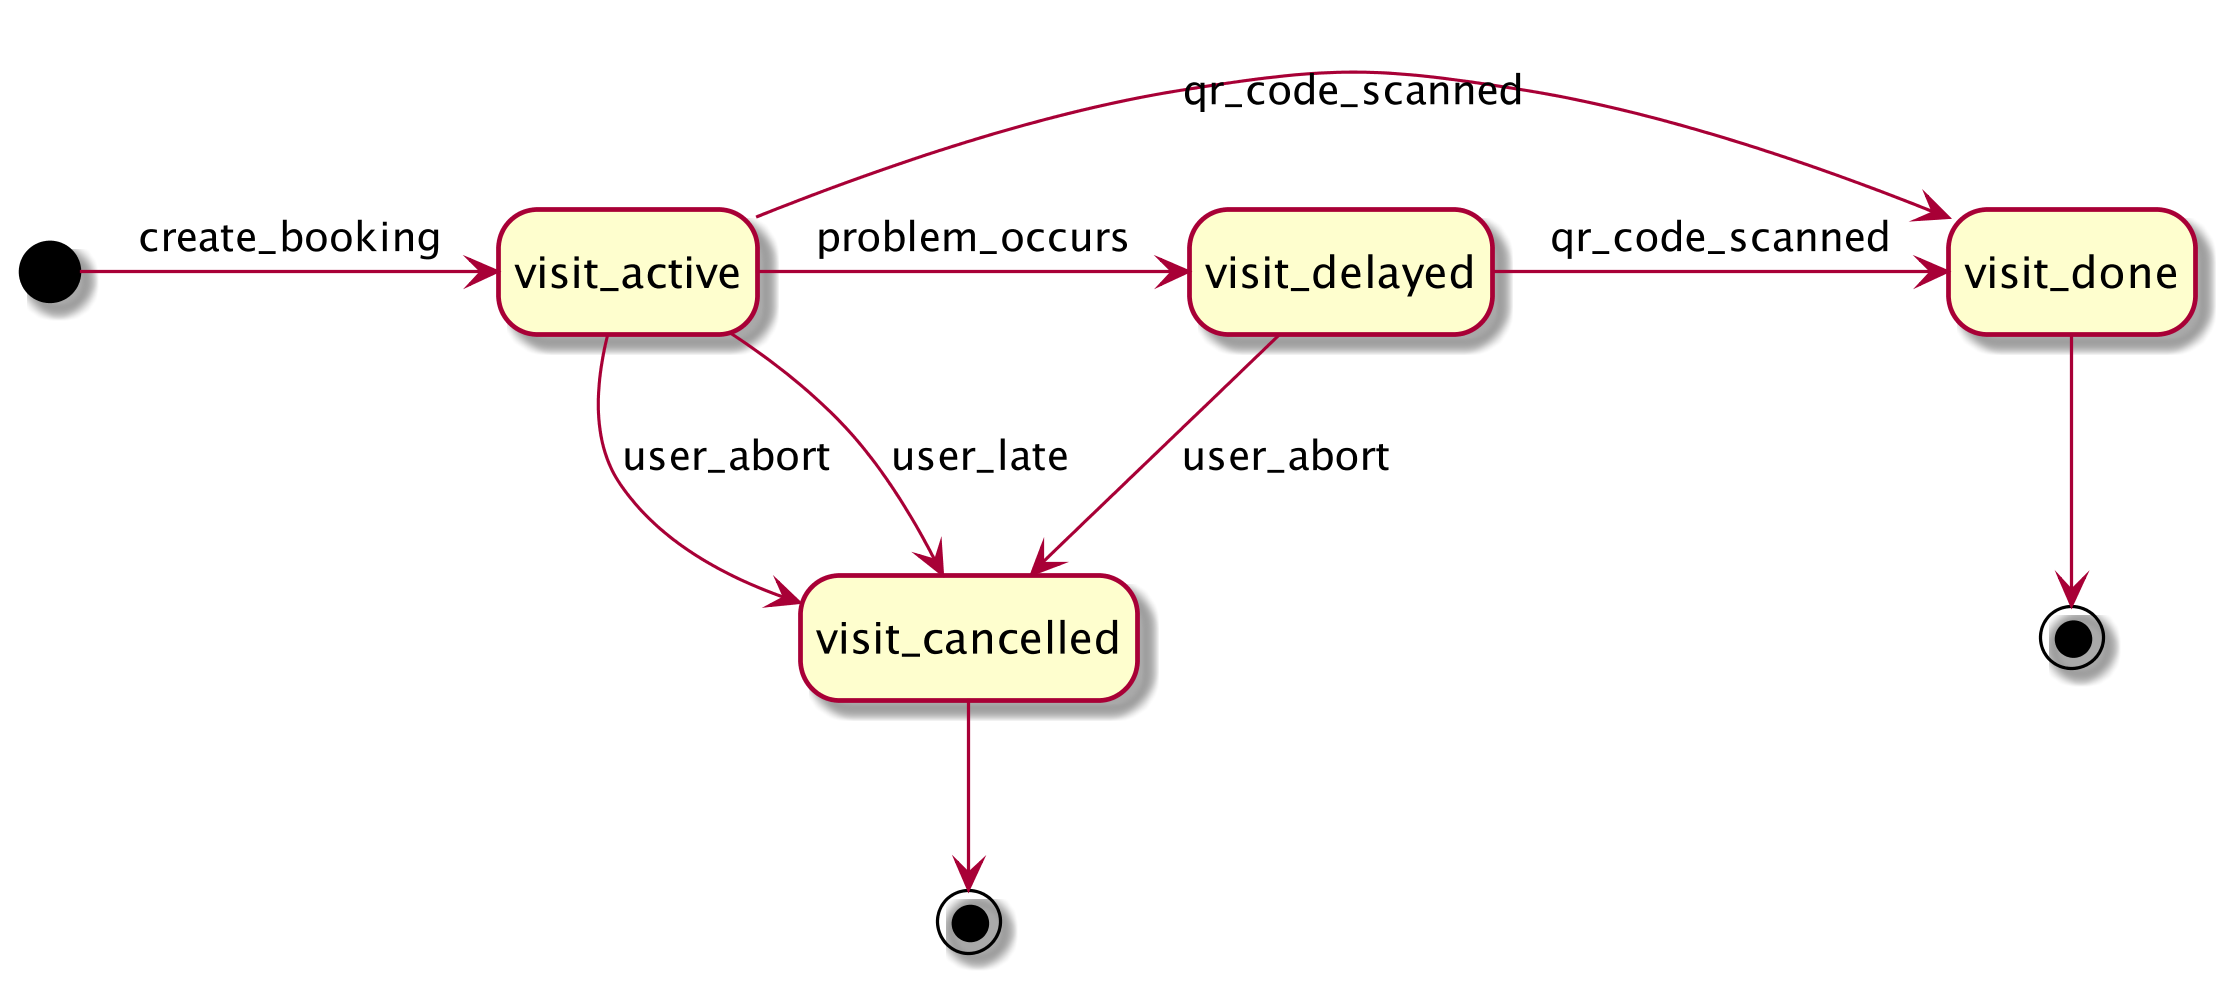
\includegraphics[width=1\textwidth]{uml/visit_state_diagram.png}
    \label{fig:visit_state_diag}
    \caption{Book a visit state diagram}
\end{figure}


\subsubsection{Scenarios}
    \begin{enumerate}[label=\Alph*.]
        \item \textbf{Customer with the mobile app arrives in time}\\
            Ian wants to buy groceries to make a cake. Ian uses CLup to get a ticket for the supermarket with the shortest queue in his area.
            The app provides Ian with a QR code and an estimate of the time when he'll be granted access to the store. 
            Ian arrives at the supermarket in the correct time slot, scans the code generated by the app and he is granted access to the store. Once he pays for his groceries the system register the exit of a user from the store. 

        \item \textbf{Customer with no knowledge on the booking system}\\
            Pino is an elderly man. Pino knows nothing about Smartphones or Computers. Pino needs to buy a cake for his
            nephew's birthday party, so he decides to go to the local supermarket. When he arrives, he notices that the doors of the supermarket
            aren't opening. He reads the sign pointing him to a totem. 
            As soon as he approaches the machine, the machine activates itself an starts speaking with a reassuring voice. 
            The machine allows Pino to get a ticket for the queue to enter the store and instructs Pino on how to do so. 
            As soon as the time is up, Pino places his ticket onto the reader beside the door of the store, and he is granted access. 

        \item \textbf{Customer cancels the reservation}\\
            Luigi, after booking a visit to the store, remembers that he had a visit to the dentist at the same time.
            Since Luigi cares about others, he cancels his reservation, freeing up a time slot to be used by other customers.

        \item \textbf{Customer is unable to provide their code}\\
            Andrea books visit and reaches the store in time, but has forgot to charge his phone, which turns off as he pulls it out of his pocket in order to scan his code.
            Andrea goes at the totem, gets a new queue ticket with a QR code and an estimate of the remaining time in queue, then he waits at an adequate distance for his turn.
        \item \textbf{Manager adjusts the number of users allowed without reservation}\\
            Ada is a store manager that notices that most of the customers at her store are elderly and do not make use of the app. She also notices that very few
            customers actually use the app, and the system is reserving too many spots for customers using the app. She navigates to the web panel of the service,
            logs in with her credentials, and navigates to the correct section, then she increase the number of customers allowed without reservation. The system
            automatically decreases the number of customers allowed by booking with the app.
        \item \textbf{Store employee creates fast-line ticket for pregnant lady}\\
            The store manager has enabled a dedicated queue for pregnant ladies and people with disabilities
            Mark is the store employee assigned to control the flow at the entrance of the store. Laura is a pregnant lady that hasn't got a reservation, but she deserves a ticket for the dedicated queue (or even instant access if possible). Laura goes to Mark and asks him to provide her with a fast-line ticket. Mark uses his credential on the totem to create a special ticket and gives it to Laura. Laura enters the store with the provided ticket and is able to get the things that she needed.         
        \end{enumerate}
\subsection{Product Functions}
The functions of Customer Line-Up can be clearly divided in two categories, based on the type of the stakeholder that is being addressed.

\subsubsection{Manager functions}
The manager is the owner of the store or store chain that is using the system.
The functions targeted at the manager regard the management of the queue and the knowledge of statistics about the behavior of the clients.
The system will let managers select the type of commercial exercise (whether single store or chain), manage independently every physical store, select the number of slots dedicated to reservation and the ones dedicated to a regular queue, as well as to create a high-priority queue for special categories of customers.
At the same time the system will provide info about the number of people who are currently in a store,
how the number of people changes over time and the average visit length.

\subsubsection{Customer functions}
The customer is the person who visits a store.
The functions targeted at the customer regard the possibility of skipping queues.
The system will let people book visits at specific time slots or queue up at the moment.
If the user is in the queue, they will be updated live with their estimated time of entrance in the store.
If the user has booked a visit, they will be notified immediately if the system realizes that
their visit has become unfeasible and automatically assign a new time or, in the worst case, cancel completely the visit.
The system will offer the possibility of creating an account and of logging in.
The system will allow the user to setup ad-hoc notification when specified conditions are met (for example a combination of store, days of the week and a timeframe).
The system will enable the user to book a visit applying filters to stores based on the following criteria: distance from the current position of the user, available days of the week and time frame of the available slots.  


\begin{comment}
\begin{itemize}
    \item Manager:
    \begin{itemize}
        \item monitor the current status of all stores
        \item obtain information on the behavior of customers
        \item adjust the maximum number of customers allowed inside a specific store
    \end{itemize}
    \item Customer:
    \begin{itemize}
        \item account:
        \begin{itemize}
            \item create a new account
            \item delete an owned existing account
            \item show the reservation history
            \item provide all information related to the account, especially
            \begin{itemize}
                \item average visit duration
                \item favorite stores
            \end{itemize}
        \end{itemize}

        \item booking:
        \begin{itemize}
            \item book a visit to the store
            \item give suggestions regarding when and where to book
            \item send notifications regarding the status of a reservation, whether it has been delayed or deleted
            \begin{itemize}
                \item send notifications via mobile app
                \item send notifications via SMS
                \item send notifications via phone call
            \end{itemize}
            \item cancel a reservation
        \end{itemize}

        \item show nearby stores and their availability
    \end{itemize}
\end{itemize}
\end{comment}

\subsection{User Characteristics}
Customers Line-Up is mainly aimed at essential and widely used services.
Because of this its audience will be wide and diversified, and the system will be easy to use and accessible in several of ways, accounting in particular for people with disabilities or people who are not familiar with technology.
On one side of the system there is the system manager (single or multiple), who will monitor how the system is used and obtain useful information.
They are usually already familiar with othe customer relationship managers and already know what to expext from a control panel.
On the other side there is the customer, who uses the system in order to avoid boring lines and to prevent contact with others.
The main categories of customer are:
\begin{itemize}
    \item \textbf{Tech-friendly}\\
        People who are familiar with modern technologies. They find it easy to navigate the menus of a complex application.
        They are able to use the system in an autonomous way and are the ones who will benefit the most from the more complex and advanced features.
    \item \textbf{Tech-unfriendly}\\
        People who are not familiar with modern technologies. They have problems navigating complex application, and are more accustomed to talking to humans.
        They might need aid using the system or misuse the system. They benefit from a system designed around clarity and simplicity, or from different, easier ways of using the system.
        This category includes people with disabilities.
\end{itemize}

The objective of Customers Line-Up is to be as inclusive as possible, providing utilities targeted at all possible users.

\subsection{Assumptions, Dependencies, and Constraints}

\subsubsection{Domain Assumptions}
\begin{enumerate}[label={[D\arabic*]}]
    \item The number of people in a store cannot go over a certain fixed amount.
    \item If an user enters the store they will exit the store before it closes.
    \item The system reliably counts (e.g. with a turnstyle, through an employee) the number of people entering and exiting the store.
    \item There's no mismatch between the real state of the store and its representation by the system.
    \item A customer cannot enter the store without using the system.
    \item External software dependencies the system relies on always provide true data and never fail.
\end{enumerate}

\subsubsection{Dependencies}
\begin{itemize}
    \item The system requires access to a third party maps API.
    \item The system needs a third party API in order to send SMS to customers' phones.
    \item The mobile app shall be deployed on major mobile phones operating systems (Android, iOS).
    \item The website requires a modern browser (no legacy browser support).
    \item The application deployed on the totem has to be compatible with its operative system.
\end{itemize}

\subsubsection{Constraints}
\begin{itemize}
    \item The system shall be compliant to local laws and regulations, in particular users data should
    be treated according to the \href{https://gdpr.eu/}{GDPR}. This means that users should be always able
    to request their data.
    \item The system should in first place limit itself to collect only
    the necessary ones to function, such as the user telephone number.
    \item To better protect the users' sensitive information, such as their telephone number, their data should
    be encrypted.
\end{itemize}